\subsection{Problem}
In modern society, the significance of physical well-being is progressively increasing. When people engage in gym workouts, it is crucial for them to ensure that their movements are executed in a proper form. Although some trainees opt to hire a personal trainer to maintain correct posture, not everyone can afford this luxury. Consequently, some individuals may fail to achieve desired results when exercising alone, and potentially cause muscle and joint damage due to incorrect movements. According to a study published in the Journal of Strength and Conditioning Research, ``improper weightlifting technique is one of the most common causes of injury in eightlifting" \cite{keogh2006injury}. Therefore, it is crucial to maintain proper form while exercising alone.
In addition, people sometimes get distracted if they tend to count the number of the movement they do while doing exercise. It will be helpful if there is a robot that can count the number of the movement and give feedback to the user.

\subsection{Solution}
Inspired by the fact \cite{li2019real}, \cite{liu2021robotics} that the role of a personal trainer can also be fulfilled by robotics, our team aim to build an automated system that acts a gym trainer. We plan to achieve our goal from both the hardware and software aspects.

The hardware components of the robot comprise a mobile platform, a control console, a display screen, and a speaker. We also plan to equip our robot with a variety of sensors, including a camera and ultrasonic radars. By utilizing a camera and ultrasonic radars, the robot is capable of determining the user’s location and distance. From the software perspective, we plan to adopt algorithms and framework such as Mediapipe to identify human movements when people are moving, compare with the existing action models, and give an performance evaluation and count the number of exercise done. The use of machine learning algorithms will enable the robot to provide more accurate feedback on the user’s performance and suggest areas for improvement. 

Overall, our solution aims to provide users with a personalized and effective gym training experience, utilizing the latest advancements in robotics and machine learning technologies. By taking a comprehensive approach to implementation, we hope to create a system that is not only effective but also efficient and easy to use.

\subsection{Visual Aid}
\begin{figure}[H]
    \centering
    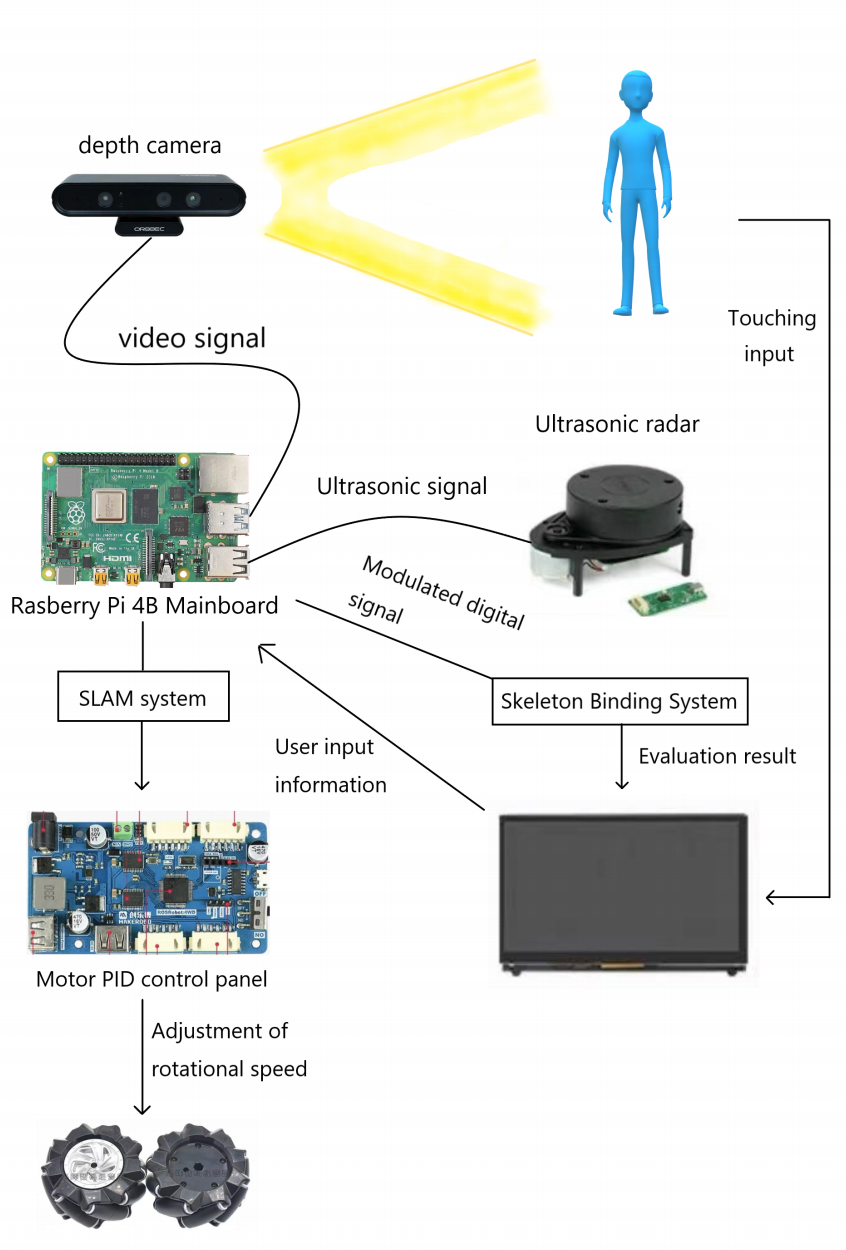
\includegraphics[width=12cm, height=17.5cm]{sections/Visual.png}
    \caption{Visual Aid}
\end{figure}


\subsection{High-Level Requirement List}
\begin{itemize}
\item The robot should be able to use KCF algorithm to track and follow the user’s location within a certain distance (2-3 meters) with the distance error smaller than 0.2 meter, using depth camera and ultrasonic radar to get the environment information. 

\item The robot should be able to recognize body key points and skeleton binding with larger than 0.95 overall high accuracy and speed (fewer than 10 seconds for one minute video), using Mask R-CNN network. 

\item The robot should be able to count and evaluate the user’s performance of two common exercising movements, such as squats and push-up.

\item The robot should be able to display the evaluation results on the display screen in a user-friendly manner.
\end{itemize}